%------------------------------------------------------%
%------------------------------------------------------%
%    Modelo de Projeto de TCC - TADS - PI 1 ( IFMS-NA) % 
% NÃO ALTERE OU APAGUE ESSAS INFORMAÇÕES
% ELAS SÃO A CONFIGURAÇÃO DO SEU ARQUIVO.
%-------------------------------------------------------
%-------------------------------------------------------


\documentclass[
	12pt,				% tamanho da fonte
	openright,			% capítulos começam em pág ímpar 
	twoside,			% para impressão em verso e anverso. Oposto a oneside
	a4paper,			% tamanho do papel. 
	%normalfigtabnum,
	%pnumromarab,
	% Opções da classe abntex2
	chapter=TITLE,		% títulos de capítulos convertidos em letras maiúsculasa
	%section=TITLE,		% títulos de seções convertidos em letras maiúsculas
	%subsection=TITLE,	% títulos de subseções convertidos em letras maiúsculas
	%subsubsection=TITLE,% títulos de subsubseções convertidos em letras maiúsculas
	% Opções do pacote babel
	english,			% idioma adicional para hifenização
    spanish,			% idioma adicional para hifenização
	brazil,				% o último idioma é o principal do documento
]{abntex2}

% ----------------------------------------------------------------
%                           PACOTES
% ----------------------------------------------------------------

		

\usepackage[utf8]{inputenc}		% O pacote inputenc é usado para que seja possível escrever textos acentuados em determinado padrão de codificação. No caso, abnTEX2 utiliza a codificação UTF8. Consulte detalhes do pacote em <http://www.ctan.org/pkg/inputenc>.
\usepackage[T1]{fontenc}		% O pacote fontenc controla a codificação das fontes usadas para impressão do documento. Consulte detalhes do pacote em <http://www.ctan.org/pkg/fontenc>.
\usepackage{times}
\usepackage{lastpage}			% Usado pela Ficha catalográfica
\usepackage{indentfirst}		% Indenta o primeiro parágrafo de cada seção.
\usepackage{xcolor,colortbl}	% Controle das cores
\usepackage{graphicx}			% Inclusão de gráficos
\usepackage{microtype} 			% para melhorias de justificação
\usepackage{hyperref}           % pacote para adicionar links internos
\usepackage{subfig}
\usepackage{epigraph}
%\usepackage[authoryear,round,longnamesfirst]{natbib}
\usepackage{url}
\usepackage{placeins}
\usepackage{multirow}
\usepackage[figuresright]{rotating}
\usepackage{chemfig}
\usepackage{amsmath}
\usepackage{amssymb}
\usepackage{enumitem}
\usepackage{bigints}
\usepackage{listings}
\usepackage{etoolbox}
\usepackage[final]{pdfpages}
\usepackage{bigstrut}
\usepackage{acronym}
\usepackage{longtable}
\usepackage{verbatim}          % pacote para adicionar comentarios em bloco
\usepackage{hypernat}
%\usepackage{titlesec}          % para permitir a alteracao em titulos

%-----------------------------------------------------
%-----------------------------------------------------
%	FLOATS: TABLES, FIGURES E CAPTIONS: CONFIGURAÇÕES
%-----------------------------------------------------

\usepackage{tabularx} % Better tables
\setlength{\extrarowheight}{3pt} % Increase table row height
\newcommand{\tableheadline}[1]{\multicolumn{1}{c}{\spacedlowsmallcaps{#1}}}
\newcommand{\myfloatalign}{\centering} % To be used with each float for alignment
\usepackage{caption}
\captionsetup{format=hang,font=small}
\usepackage{subfig}

%----------------------------------------------------
%	LIST ENUMERATION
%----------------------------------------------------

\renewcommand{\labelenumii}{\theenumii}
\renewcommand{\theenumii}{\theenumi.\arabic{enumii}.}
% ---
% Pacotes adicionais, usados apenas no âmbito do Modelo Canônico do abnteX2
% ---
\usepackage{lipsum}				% para geração de dummy text
% ---

% ---
% Pacotes de citações
% ---
\usepackage[brazilian,hyperpageref]{backref}	 % Paginas com as citações na bibl
\usepackage[alf,abnt-emphasize=bf]{abntex2cite}  % Citações padrão ABNT

% ------------------------------------------------------
%             CONFIGURAÇÕES DOS PACOTES
% ------------------------------------------------------

% ---
% Configurações do pacote backref
%
% Para desativar, tire o comentário de \begin{comment} e \end{comment} das próximas linhas e comente a linha \usepackage[brazilian,hyperpageref]{backref}
% acima.
% ---

%\begin{comment}
% ---
% Configurações do pacote backref
% Usado sem a opção hyperpageref de backref
\renewcommand{\backrefpagesname}{}
%\renewcommand{\backrefpagesname}{Citado na(s) página(s):~}
% Texto padrão antes do número das páginas
\renewcommand{\backref}{}
% Define os textos da citação
 \renewcommand*{\backrefalt}[4]{
% 	\ifcase #1 %
% 	Nenhuma citação no texto.%
% 	\or
% 	Citado na página #2.%
% 	\else
% 	Citado #1 vezes nas páginas #2.%
% 	\fi}%
}
% ---
%\end{comment}


% listagens
\definecolor{corComentario}{RGB}{150,150,150}
\definecolor{corString}{RGB}{206,123,0}
\definecolor{corPalavraChave}{RGB}{0,0,230}

\lstset{
	numbers=left,
	stepnumber=1,
	firstnumber=1,
	numberstyle=\footnotesize,
	extendedchars=true,
	breaklines=true,
	lineskip=0pt,
	frame=tb,
	basicstyle=\ttfamily\footnotesize,
	showstringspaces=false,
	stringstyle=\color{corString},
	commentstyle=\color{corComentario},
	keywordstyle=\color{corPalavraChave}
}

\newcolumntype{Y}{>{\centering\arraybackslash}X}

\newcommand{\ano}[1]{\def \oano {#1}}
\newcommand{\imprimirano}{\oano}

\newcommand{\mes}[1]{\def \omes {#1}}
\newcommand{\imprimirmes}{\omes}

\newcommand{\subtitulo}[1]{\def \osubtitulo {#1}}
\newcommand{\imprimirsubtitulo}{\osubtitulo}

\newcommand{\area}[1]{\def \aarea {#1}}
\newcommand{\imprimirarea}{\aarea}

\renewcommand{\coorientador}[1]{\def \ocoorientador {#1}}
\renewcommand{\imprimircoorientador}{\ocoorientador}

\newcommand{\grau}[1]{\def \ograu {#1}}
\newcommand{\imprimirgrau}{\ograu}

\newcommand{\curso}[1]{\def \ocurso {#1}}
\newcommand{\imprimircurso}{\ocurso}

\usepackage{edicoes}

%--------------------------------------------
%----------------Não Alterar-----------------
\curso{TECNOLOGIA EM ANÁLISE E DESENVOLVIMENTO DE SISTEMAS}
\grau{Tecnólogo em Análise e Desenvolvimento de Sistemas}
\tipotrabalho{Trabalho de Conclusão de Curso}
\local{NOVA ANDRADINA - MS}
\instituicao{%
	INSTITUTO FEDERAL DE EDUCAÇÃO, CIÊNCIA E TECNOLOGIA DE MATO GROSSO DO SUL
	CÂMPUS NOVA ANDRADINA
}
\preambulo{\imprimirtipotrabalho\ apresentado ao Instituto Federal de Educação, Ciência e Tecnologia de Mato Grosso do Sul – Câmpus Nova Andradina – como um dos requisitos para a obtenção do título de \imprimirgrau.\\
}

% ---

% ---
% Configurações de aparência do PDF final
% ---

% alterando o aspecto da cor azul
\definecolor{blue}{RGB}{41,5,195}

% informações do PDF
\makeatletter
\hypersetup{
	%pagebackref=true,
	pdftitle={\@title}, 
	pdfauthor={\@author},
	pdfsubject={\imprimirpreambulo},
	pdfcreator={Nome Completo},
	pdfkeywords={Palavra chave 1}{Palavra chave 2}{Palavra chave 3}{Palavra chave n}, 
	colorlinks=true,       		% false: boxed links; true: colored links
	linkcolor=black,          	% color of internal links
	citecolor=black,       		% color of links to bibliography
	filecolor=black,      		% color of file links
	urlcolor=blue,
	bookmarksdepth=4
}
\makeatother
% --- 

% ---
% Comandos do autor
% ---
% para ajustar o tamanho da fonte no cabeçalho

% Agradecimentos
\renewenvironment{agradecimentos}[1][\agradecimentosname]{%
    %\ABNTEXchapterfont{\large{#1}}
   \pretextualchapter{\large{#1}}
  }{\PRIVATEclearpageifneeded}
% ---

\renewenvironment{resumo}[1][\resumoname]{%
   \PRIVATEbookmarkthis{#1}
   \renewcommand{\abstractnamefont}{\chaptitlefont}
   \renewcommand{\abstractname}{\ABNTEXchapterupperifneeded{\large{#1}}}
   \begin{abstract}
  }{\end{abstract}\PRIVATEclearpageifneeded}

% comando para inserir autor e ano
\newcommand{\citeauthorandyear}[1]{\citeauthoronline{#1} (\citeyear{#1})}

% ---
% Novo list of (listings) para Quadros
% ---

\newcommand{\quadroname}{Quadro}
\newcommand{\listofquadrosname}{Lista de Quadros}

\newfloat[chapter]{quadro}{loq}{\quadroname}
\newlistof{listofquadros}{loq}{\listofquadrosname}
\newlistentry{quadro}{loq}{0}

% configurações para atender às regras da ABNT
\setfloatadjustment{quadro}{\centering}
\counterwithout{quadro}{chapter}
\renewcommand{\cftquadroname}{\quadroname\space} 
\renewcommand*{\cftquadroaftersnum}{\hfill--\hfill}

% Configuração de posicionamento padrão:
\setfloatlocations{quadro}{hbtp}

% ---
% Fontes padroes de part, chapter, section, subsection e subsubsection
\renewcommand{\ABNTEXchapterfont}{\large\bfseries}
\renewcommand{\ABNTEXchapterfontsize}{\large}

\renewcommand{\ABNTEXpartfont}{\normalfont}
\renewcommand{\ABNTEXpartfontsize}{\ABNTEXchapterfontsize}

\renewcommand{\ABNTEXsectionfont}{\normalfont\MakeUppercase}
\renewcommand{\ABNTEXsectionfontsize}{\Large}

\renewcommand{\ABNTEXsubsectionfont}{\normalfont\bfseries}
\renewcommand{\ABNTEXsubsectionfontsize}{\normalsize}

\renewcommand{\ABNTEXsubsubsectionfont}{\normalfont\bfseries}
\renewcommand{\ABNTEXsubsubsectionfontsize}{\normalsize\bfseries}

\renewcommand{\ABNTEXsubsubsubsectionfont}{\normalfont}
\renewcommand{\ABNTEXsubsubsubsectionfontsize}{\normalsize}
% ---




% ------------------------------------------------------------
%           Espaçamentos entre linhas e parágrafos 
% ------------------------------------------------------------

% O tamanho do parágrafo é dado por:
\setlength{\parindent}{1.3cm}

% Controle do espaçamento entre um parágrafo e outro:
\setlength{\parskip}{0.2cm}  % tente também \onelineskip

% indicando o caminha das imagens para todo o documento.
\graphicspath{ {imagens/} }

% ---------------------------------------------------------
%                   Compila o indice
% ---------------------------------------------------------

% Você pode customizar o nível de divisões que o sumário pode listar com a macro \settocdepth{hnome da subdivisãoi}, sendo nome da subdivisão UM dos valores: chapter, part, section, subsection, subsubsection
\settocdepth{subsection}

\makeindex
% ---

%===========================================
%                 CABEÇALHO
%===========================================

%%criar um novo estilo de cabeçalhos e rodapés
\makepagestyle{meuestilo}
  %%cabeçalhos
  \makeevenhead{meuestilo} %%pagina par
     {\thepage}         % esquerda
     {}         % centro
     {} % direita
  \makeoddhead{meuestilo} %%pagina ímpar ou com oneside
     {} % esquerda
     {}         % centro
     {\thepage}         % direita
  %\makeheadrule{meuestilo}{\textwidth}{\normalrulethickness} %linha
  %% rodapé
  %\makeevenfoot{meuestilo}
     %{rodapé par à esquerda} %%pagina par
     %{centro \thepage}
     %{\thepage} 
  %\makeoddfoot{meuestilo} %%pagina ímpar ou com oneside
     %{rodapé ímpar/onside à esquerda}
     %{centro \thepage}
     %{\thepage}


%===========================================
%               FIM CABEÇALHO
%===========================================


% ------------------------------------------------------
%                 INÍCIO DO DOCUMENTO
% ------------------------------------------------------
\begin{document}

% Seleciona o idioma do documento (conforme pacotes do babel)
%\selectlanguage{english}
\selectlanguage{brazil}

%\pagestyle{plain}
% Retira espaço extra obsoleto entre as frases.
\frenchspacing 

% ---------------------------------------------------
%   INSERIR PÁGINAS DOS ELEMENTOS PRÉ-TEXTUAIS
% -----------------------------------------------------
% \pretextual

% ---
% CapA
%\imprimircapa
\begin{center}
	
	%\center
	\ABNTEXchapterfont\bfseries\large\textsc{\textbf{\imprimirinstituicao}}
	\vspace{1.0cm}
    
    \ABNTEXchapterfont\large\textsc{\textbf{\imprimircurso}}
	\vspace{3.5cm}
	
    \ABNTEXchapterfont\large\textsc{\textbf{\imprimirautor}}
	\vspace{3.5cm}
	
    \ABNTEXchapterfont\large\textsc{\textbf{\imprimirtitulo\ifdef{\osubtitulo}{:}{}}}
    
    \ifdef{\osubtitulo}{\ABNTEXchapterfont\large\textbf{\imprimirsubtitulo}}{}
	\vfill
	
	\SingleSpacing
	\large\textsc{\textbf{\imprimirlocal}}\\
	\large\textsc{\textbf{\imprimirano}}

	%\vspace*{2cm}
	
\end{center}

\cleardoublepage
% ---
% Folha de rosto
%\imprimirfolhaderosto*
\begin{center}
   	
   	\ABNTEXchapterfont\large\textsc{\textbf{\imprimirautor}}
   	\vspace{6.5cm}
   	
    \ABNTEXchapterfont\large\textsc{\textbf{\imprimirtitulo}}\ifdef{\osubtitulo}{:}{}
                           
    \ifdef{\osubtitulo}{\ABNTEXchapterfont\large\textbf{\imprimirsubtitulo}}{}
   	\vspace{1.5cm}
   	   	
   	\hspace{.5\textwidth}
   	\begin{minipage}{.4\textwidth}
   		\SingleSpacing
   		\footnotesize\imprimirpreambulo
   		
   		%\vspace{\onelineskip}
   		
   		\textbf{Orientador:} \imprimirorientador
   		
        \ifdef{\ocoorientador}{
     		\vspace{\onelineskip}
   		
    	\textbf{Coorientador:} \imprimircoorientador
        }{}
   		
   	\end{minipage}%
    \vfill
   	
   	\SingleSpacing
   	\normalsize\textsc{\textbf{\imprimirlocal}}\\
   	\normalsize\textsc{\textbf{\imprimirano}}
   	
   	%\vspace*{2cm}
   	
\end{center}
% ---
% Inserir a ficha catalográfica
% --- para ficha, retire o % da linha de baixo.
%%
% Este é um exemplo de ficha catalográfica.
%
% A ficha catalográfica final deve ser requisitada pelo aluno e inserida neste
% documento para a entrega da versão final.
%

\begin{fichacatalografica}
    
\includepdf{fichaCatalografica/ficha_catalografica}
\end{fichacatalografica}

% Inserir folha de aprovação
% --- para inserir a folha de aprovação retire o % da linha de baixo.
%%
% Este é um exemplo de folha de aprovação.
%
% A folha de aprovação final será inserida pelo Coordenador do Curso.
%

\begin{folhadeaprovacao}
	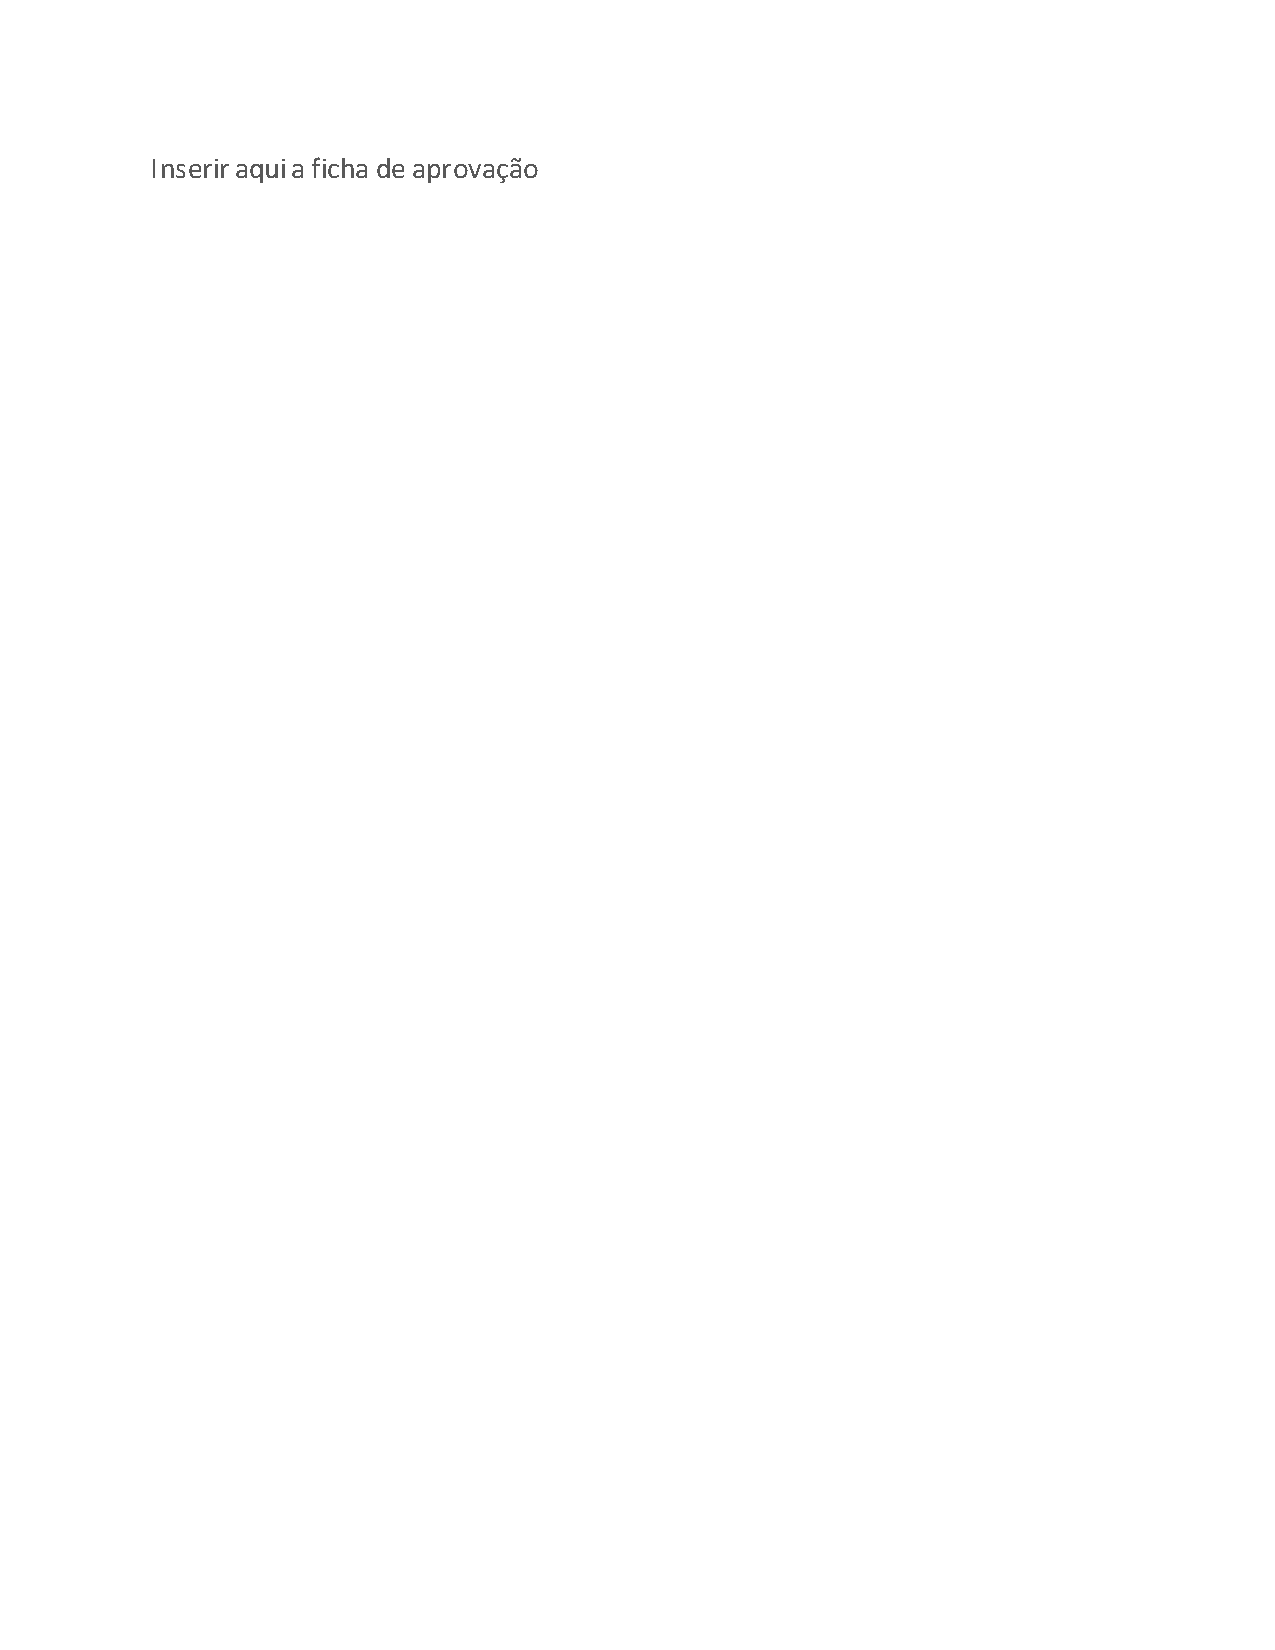
\includepdf{folhaAprovacao/folha_aprovacao}
\end{folhadeaprovacao}
% ---
% Dedicatória
% --- para inserir dedicatória, retire o % da linha de baixo.
% \begin{dedicatoria}
	\vspace*{\fill}
	\centering
	\noindent
	\textit{Dedicatória (Opcional). Não digite a palavra Dedicatória. Texto no qual o autor do trabalho oferece homenagem ou dedica o seu trabalho a alguém (não usar ponto final)}
    \vspace*{\fill}
\end{dedicatoria}
% ---
% Agradecimentos
\begin{agradecimentos}
	A descrição dos agradecimentos é opcional.
	Caso você não deseje inserir agradecimento, já até a página de configuração (monografia\_config) e insira um comentário (\%) na chamada da página.
	
	Caso faça os agradecimentos, se atente em seguir algumas dicas de boa escrita:
	
	\begin{itemize}
	    \item Cite as pessoas que foram responsáveis pela execução do seu trabalho, porém se atente em agradecer brevemente, para não ficar muito extenso;
	    \item Cite a instituição e possíveis recursos utilizados que te ajudaram a terminar o projeto;
	    \item Caso tenha fomento, cite um breve agradecimento;
	    \item Caso resolva fazer agradecimentos pessoais, evite citar muitas pessoas, faça um breve agradecimento de modo geral, para evitar um texto muito carregado;
	    \item Agradeça ao seu orientador e coorientador e outros colaboradores ligados ao projeto;
	    \item Evite expressões tais quais "obrigado por não surtar" ;  "esse TCC me fez passar muito nervoso" , "agradeço aos meus cachorros", "agradeço ao meu psiquiatra que me receitou Rivotril".. TCC é um documento do aluno que será registrado na biblioteca, podendo ser publicado em teses online, portanto, por mais que seja brincadeira, não é legal inserir esse tipo de declaração. Sem contar que a banca pode ter uma impressão negativa de você.
	\end{itemize}
\end{agradecimentos}
% ---
% Epígrafe
% --- para inserir Epígrafe, retire o % da linha de baixo
% \begin{epigrafe}
	
	\vspace*{\fill}
	Epígrafe (Opcional). Pensamentos retirados de um livro, uma música, um poema, normalmente relacionado ao tema do trabalho, seguida de indicação de autoria. As epígrafes podem ser colocadas também nas folhas de abertura de cada capítulo.  
    
	\epigraph{``\emph{Any fool can write code that a computer can understand. Good programmers write code that humans can understand}''.}{Martin Fowler}
	
\end{epigrafe}
% ---
% Resumos
\begin{resumo}

%\noindent{SILVA, João da. \textbf{Título do trabalho de conclusão de curso em negrito}. Nº de fls. TCC (Trabalho de Conclusão de Curso). Instituto Federal de Mato Grosso do Sul – IFMS. Tecnologia em Análise e Desenvolvimento de Sistemas, Câmpus Nova Andradina, MS. 2018.}

%\setlength{\absparsep}{18pt} % ajusta o espaçamento dos parágrafos do resumo
%\vspace{1.5cm}
	
A acessibilidade digital é um desafio crucial em um mundo cada vez mais conectado, especialmente para pessoas com deficiência visual. Este trabalho apresenta o desenvolvimento de um aplicativo multiplataforma assistivo capaz de capturar imagens do ambiente e descrevê-las em áudio, utilizando modelos de linguagem de grande porte (LLMs) de código aberto. O aplicativo integra recursos de visão computacional e síntese de voz (Text-to-Speech - TTS), promovendo maior autonomia para usuários com deficiência visual. A metodologia incluiu o benchmark de três modelos de IA (Qwen 2.5, llava v1.6 Mistral e Llama 3.2 Vision), avaliados com base em métricas de latência, qualidade textual (BERTScore e ROUGE-L) e testes práticos em cenários reais. Os resultados demonstraram que o modelo Qwen 2.5 apresentou o melhor equilíbrio entre precisão descritiva e desempenho em tempo real. O protótipo desenvolvido evidencia o potencial da IA para ampliar a inclusão digital, destacando-se como uma solução inovadora para a melhoria da qualidade de vida de pessoas com deficiência visual.

	\vspace{\onelineskip}
	
	\textbf{Palavras-chave}: Acessibilidade Digital, Tecnologia Assistiva, Modelos de Linguagem Multimodais, Visão Computacional, Inclusão Social.
	
\end{resumo}
\begin{resumo}[Abstract]
	
	\begin{otherlanguage*}{english}
		
	Digital accessibility is a crucial challenge in an increasingly connected world, especially for people with visual impairments. This paper presents the development of a cross-platform assistive application capable of capturing environmental images and describing them in audio using open-source large language models (LLMs). The application integrates computer vision and text-to-speech (TTS) technologies, promoting greater autonomy for visually impaired users. The methodology included benchmarking three AI models (Qwen 2.5, llava v1.6 Mistral e Llama 3.2 Vision), evaluated based on latency metrics, textual quality (BERTScore and ROUGE-L), and practical tests in real-world scenarios. The results showed that the Qwen 2.5 model achieved the best balance between descriptive accuracy and real-time performance. The developed prototype demonstrates the potential of AI to enhance digital inclusion, standing out as an innovative solution to improve the quality of life for visually impaired individuals.
	
    \textbf{Keywords}: Digital Accessibility, Assistive Technology, Multimodal Language Models, Computer Vision, Social Inclusion.
		
	\end{otherlanguage*}

\end{resumo} 
% ---
% inserir lista de ilustrações
% ---
\renewcommand{\listfigurename}{\large{Lista de figuras}}
\pdfbookmark[0]{\listfigurename}{lof}
\listoffigures*  % O * remove esse item do indice
\cleardoublepage
% ---
% inserir lista de tabelas
% ---
\renewcommand{\listtablename}{\large{Lista de Tabelas}}
\pdfbookmark[0]{\listtablename}{lot}
\listoftables*
\cleardoublepage
% ---
% ---
% inserir lista de quadros
% --- Para inserir lista de quadros, tire o % da linha de baixo
% \pdfbookmark[0]{\listofquadrosname}{loq}
% \listofquadros*
% \cleardoublepage
% ---
% inserir lista de abreviaturas e siglas
% --- para inserir lista de Abreviaturas e Siglas, retire o % da linha de baixo
% \begin{siglas}
	\item AAAAAAAAAA
\end{siglas}


%*******************************************************
%                Acronimos
%*******************************************************
    %\phantomsection 
    %\refstepcounter{dummy}
    %\pdfbookmark[1]{Acronyms}{acronyms}
    %\markboth{\spacedlowsmallcaps{Acronyms}}{\spacedlowsmallcaps{Acronyms}}
    %\chapter*{\large{Acrônimos}}
    %\begin{acronym}[UML]
        %\acro{XXX}{nome aqui}
    %\end{acronym} 
    
    %\cleardoublepage
% ---

% ---
% inserir lista de símbolos
% ---
% \begin{simbolos}
	\item[$\alpha$] Letra grega minúscula Alfa
	\item[$\beta$] Letra grega minúscula Beta
\end{simbolos}
% ---

% ------------------------------------
% INSERIR SUMÁRIO
% -----------------------------------
\renewcommand{\contentsname}{\large{SUMÁRIO}}

\pdfbookmark[0]{\contentsname}{toc}
\tableofcontents*
\cleardoublepage
% ---

% ----------------------------------------------
%             ELEMENTOS TEXTUAIS
%           INSERIR NOVOS ARQUIVOS
% ----------------------------------------------
% cada um desses comandos a baixo montam uma seção de capítulos do nosso documentos na hora da compilação.
% note que eles foram chamados com a ordem que eles aparecerão no documento final. Ideal é que no momento da criação, sejam renomeados de maneira lógica, numerando o capítulo e a seção.

\textual
\pagestyle{meuestilo}
\chapter{Introdução}

A acessibilidade digital tem se tornado um tema de crescente importância em um mundo cada vez mais conectado. O desenvolvimento tecnológico, nos últimos anos, tem despertado a atenção do mundo todo, especialmente quando o assunto trata-se de Inteligência Artificial (IA). Porém, mesmo em um mundo conectado, o desenvolvimento de tecnologias assistivas ainda caminha a passos lentos, levando anos para chegarem às pessoas com deficiência, especialmente aos deficientes visuais, que, por não terem visão ou terem, porém, limitada, são prejudicados no contato com recursos inovadores existentes atualmente. 

Segundo dados da \citeonline{WHO2023}, estima-se que pelo menos 2,2 bilhões de pessoas em todo o mundo vivenciam algum grau de deficiência visual, o que ressalta a necessidade de soluções tecnológicas específicas para esse público, visando a melhoria da qualidade de vida e, também, o contato com tecnologias inovadoras, como a IA. No contexto brasileiro, o Instituto Brasileiro de Geografia e Estatística (IBGE) aponta que mais de 6 milhões de pessoas têm algum nível de deficiência visual, o que evidencia a expressividade dessa população, reforçando o caráter urgente de iniciativas que promovam a inclusão. Embora diversos recursos digitais e físicos já existam para auxiliar pessoas cegas ou com baixa visão, ainda há lacunas quanto a ferramentas de reconhecimento de ambientes em tempo real por meio de dispositivos móveis.

Frente a esse cenário, o presente trabalho propõe o desenvolvimento de um aplicativo multiplataforma, capaz de capturar imagens do ambiente e descrevê-las em áudio por meio de técnicas de IA, promovendo a inclusão tecnológica e, além disso, melhorando a qualidade de vida de deficientes visuais. De acordo com \citeonline{silvaneto2024tecnologias}, a IA surge como um meio promissor para ampliar o acesso ao conhecimento, eliminar barreiras e melhorar a experiência acadêmica de grupos historicamente excluídos, como pessoas com deficiência, minorias étnicas e socioeconômicas. Nesse sentido, a proposta está alinhada às demandas atuais de inclusão e às oportunidades tecnológicas propiciadas pela evolução da IA, especialmente ao desenvolvimento dos modelos de linguagem de grande porte (do inglês, Large Language Models - LLMs), onde muitos são disponibilizados de forma gratuita, com o código aberto, em plataformas como o Hugging Face.

Desta forma, dada a crescente popularização dos smartphones e a melhoria contínua dos recursos de câmera embutidos nesses dispositivos, caminhos foram abertos para soluções inovadoras no campo da visão computacional. Não obstante, não podemos encarar a acessibilidade como um recurso adicional da tecnologia, mas como uma parte fundamental do desenvolvimento, visando garantir o acesso a qualquer grupo que a utilize. Assim, o desenvolvimento de aplicativos que traduzem informações visuais em descrições textuais e, posteriormente, em áudio, pode transformar a forma como pessoas com deficiência visual interagem com o ambiente ao seu redor.

A relevância deste estudo decorre do compromisso social de promover inclusão e autonomia a grupos historicamente sub-representados na evolução tecnológica. Além dos dados estatísticos já mencionados, há também uma motivação acadêmica, pois o uso de modelos de código livre de LLM para descrever imagens em tempo real é um tema ainda em consolidação na literatura científica, onde muitos estudos optam por usar modelos já renomados no mercado, porém proprietários. De acordo com \citeonline{lecun2015deeplearning}, o aumento da capacidade computacional, a disponibilidade de grandes bases de dados e o desenvolvimento de ferramentas de análise de dados impulsionam significativamente o progresso em redes neurais profundas, podendo contribuir para existirem modelos cada vez mais robustos. Todavia, ainda há desafios relacionados à latência, ao custo computacional e à efetiva acurácia das legendas geradas.

Assim, ao comparar diferentes modelos de linguagem pré-treinados (por exemplo, Qwen2.5-VL-7B-Instruct, Llama-3.2-11B-Vision-Instruct e o llava-v1.6-mistral-7b-hf), este trabalho busca evidenciar pontos fortes e limitações de cada abordagem, contribuindo para a consolidação de uma prática fundamentada na seleção e no emprego de soluções de IA em projetos de acessibilidade. Desta forma, este trabalho tem como objetivo desenvolver um aplicativo móvel que possibilite a descrição em áudio de elementos do ambiente para pessoas com deficiência visual, valendo-se de um servidor para processamento de imagens por meio de LLMs de código livre. Assim, como resultado final, será desenvolvida uma tecnologia assistiva que poderá contribuir fortemente para a melhoria da qualidade de vida de deficientes visuais e, além disso, proporcionar o uso de tecnologias inovadoras da atualidade.

Para alcançar esse objetivo, este trabalho está detalhado em 5 capítulos, além desta introdução, que buscou apresentar resumidamente sobre a problemática, além de discorrer sobre o objetivo geral do desenvolvimento.

No Capítulo 2, que trata do Referencial Teórico, valeu-se de uma pesquisa detalhada acerca dos conceitos de acessibilidade, tecnologias assistivas, visão computacional e do funcionamento de modelos de linguagem de grande porte, além de explorar brevemente questões sobre Text-to-Speech. Esta foi realizada por meio de ferramentas como o Periódicos Capes, Google Acadêmico e demais repositórios de trabalhos da área. 

Em seguida, no Capítulo 3 é apresentada a Metodologia, onde os métodos, ferramentas e procedimentos adotados para o desenvolvimento do aplicativo, incluindo a estratégia de benchmark dos diferentes modelos de IA, são detalhados. 

Já os Resultados e Discussões, que estão no Capítulo 4, descrevem os resultados obtidos nos testes práticos e no benchmark, analisando as métricas de desempenho e a usabilidade da solução. 

Por fim, a Conclusão, no Capítulo 5, retoma os objetivos iniciais, faz considerações finais sobre o trabalho realizado e sugere futuros aprimoramentos, dando encerramento ao trabalho.


\chapter{Objetivos}  \label{cap:02}

% Para a Banca Final, lembre-se de conversar com o orientador sobre suprimir esse capítulo já que ele terá sido cumprido, e inserí-lo na Introdução em modo Parágrafo. 
% Não apague esse comentário.


\section{Objetivo Geral}

O objetivo geral do trabalho é o elemento que resume e apresenta a ideia central do trabalho acadêmico. Normalmente é redigido em uma frase, utilizando o verbo no infinitivo. 

% textbf é um comando que deixa o texto em negrito
\textbf{Exemplo:} Detalhar o presente modelo de escrita para a produção do Trabalho de Conclusão de Curso.\\

\section{Objetivos Específicos}

% textit é um comando que deixa o texto em itálico
Os objetivos específicos definem os diferentes pontos a serem abordados, visando confirmar as hipóteses e concretizar o objetivo geral. Em suma, são as ações que serão desenvolvidas a fim de que se alcance o \textit{objetivo geral}. Devem ser escritos no infinitivo.

\textbf{Exemplo:}

\begin{itemize}
    \item Realizar a revisão bibliográfica sobre TCC;
    \item Criar um Tutorial sobre a utilização do Overleaf;
    \item Aplicar os conhecimentos adquiridos para edição de documentos.
\end{itemize}
\chapter{Referencial Teórico}  \label{cap:02}

O referencial teórico tem como objetivo fundamentar este estudo a partir de conceitos e pesquisas já consolidadas na literatura científica. Por meio da revisão de trabalhos acadêmicos, artigos e documentos técnicos, esta seção apresenta as principais bases conceituais relacionadas ao desenvolvimento deste projeto.

Inicialmente, são abordados aspectos fundamentais sobre acessibilidade e deficiência visual, destacando a importância da tecnologia assistiva para promover inclusão social. Em seguida, discutem-se as principais tecnologias de apoio utilizadas atualmente, incluindo soluções baseadas em visão computacional e inteligência artificial. Também são explorados conceitos relacionados a LLMs e sua aplicação na descrição automática de imagens, além de métricas de avaliação da qualidade das descrições geradas.

Por fim, são detalhadas as tecnologias de reconhecimento e síntese de fala (Speech-to-Text e Text-to-Speech), essenciais para a interface acessível do sistema proposto. Essas discussões servirão como base para a construção e análise do modelo desenvolvido, garantindo alinhamento com os avanços mais recentes na área.

\section{Acessibilidade e Deficiência Visual}

A acessibilidade digital refere-se à capacidade de indivíduos, independentemente de suas habilidades ou deficiências, acessarem e interagirem com informações e serviços disponíveis no ambiente digital. \citeonline{Torres2002} destacam que a acessibilidade no espaço digital envolve a adaptação de conteúdos e interfaces para garantir que pessoas com diferentes tipos de deficiência possam utilizá-los de forma eficaz.

No contexto das pessoas com deficiência visual, a acessibilidade digital é particularmente desafiadora. Conforme destacam \citeonline{Torres2002}, “as barreiras arquitetônicas não são o maior obstáculo enfrentado pelas pessoas portadoras de deficiência. O maior obstáculo está no acesso à informação e, consequentemente, a aspectos importantes relacionados à informação, como a educação, o trabalho e o lazer”. Desta forma, é evidente que se faz necessário melhorias nas tecnologias existentes para a distribuição e acesso das pessoas deficientes, como dito por \citeonline{romeo2019}, que analisam o uso de diferentes tecnologias para acesso a conteúdos digitais por pessoas com deficiência visual e sugerem melhorias nas recomendações existentes para a concepção de \textit{websites} acessíveis. Deste modo, com a evolução não somente dos \textit{websites}, mas também de todas as tecnologias, a melhoria da acessibilidade para as pessoas deficientes seria nítida.

\subsection{Dados e Estatísticas sobre a População com Deficiência Visual}

Compreender a dimensão da população com deficiência visual é crucial para justificar a relevância de soluções tecnológicas acessíveis, para que, como exposto anteriormente, a acessibilidade em ambientes digitais passe por uma melhora significativa e contribua para o acesso de todos os grupos da sociedade. \citeonline{Castro2008} conduziram um estudo que descreve a prevalência e os fatores associados às deficiências visuais, auditivas e físicas no Brasil, constatando que 68\% do público entrevistado possuía algum tipo de deficiência visual, sendo a dificuldade de enxergar a principal deficiência referida e, como um dos principais fatores agravantes, o envelhecimento, conforme apresentado pelos autores. Fica claro, portanto, que este público merece atenção redobrada, dado que, segundo o \citeonline{ibgecenso2022}, em 2022 o índice de envelhecimento da população brasileira chegou a 80,0, indicando que há 80 pessoas idosas para cada 100 crianças de 0 a 14 anos, mas, comparado a 2010, o índice de envelhecimento era menor, correspondendo a 44,8, evidenciando um aumento de 78,5\%. Esses números corroboram para que a acessibilidade digital seja um ponto de discussão sério e fundamental para o desenvolvimento da inclusão digital.

Além disso, o IBGE tem desempenhado um papel fundamental na coleta e análise de dados relacionados à população com deficiência no Brasil. A produção e divulgação dessas informações são essenciais para embasar políticas públicas e iniciativas voltadas à inclusão social. A coleta de informações ocorre por meio de pesquisas como a Pesquisa Nacional de Saúde (PNS) de 2019, a Pesquisa Nacional por Amostra de Domicílios Contínua (PNAD Contínua) de 2022 e o Censo Demográfico, cada uma com metodologias e objetivos específicos. Segundo \citeonline{Botelho2024}, “as pesquisas conduzidas pelo IBGE adotam as recomendações do Grupo de Washington de Estatísticas sobre Deficiência, mas empregam questionários distintos, o que demanda atenção dos usuários desses dados”. Esse fator evidencia a complexidade na interpretação dos indicadores e destaca a necessidade de critérios padronizados para garantir a comparabilidade ao longo do tempo. O artigo também ressalta que as pessoas com dificuldades mais severas são as que enfrentam os maiores desafios no acesso à educação e ao mercado de trabalho, o que reforça a importância de políticas públicas baseadas em dados precisos. Tais informações são fundamentais não apenas para o desenvolvimento de políticas sociais, mas também para a criação de tecnologias assistivas que possam atender às demandas dessa parcela da população.

\subsection{Panorama de Leis e Normas}

A legislação brasileira tem avançado significativamente na promoção da inclusão e acessibilidade para pessoas com deficiência visual, estabelecendo diretrizes que garantem o acesso igualitário a diversos aspectos da vida em sociedade, incluindo a educação, o trabalho e o lazer. A Lei Brasileira de Inclusão da Pessoa com Deficiência (Lei nº 13.146/2015), também conhecida como Estatuto da Pessoa com Deficiência, representa um marco regulatório importante, pois estabelece diretrizes para garantir acessibilidade em diversas esferas, incluindo educação, transporte, comunicação e tecnologia. Segundo \citeonline{Bruno2019}, a política nacional de inclusão digital tem se mostrado essencial para eliminar barreiras atitudinais e tecnológicas, proporcionando autonomia e participação ativa na sociedade para pessoas com deficiência visual. A acessibilidade digital, nesse contexto, é reconhecida como um direito fundamental, assegurando que todos os cidadãos tenham acesso igualitário às informações e oportunidades disponíveis no ambiente digital.

Além disso, a Política Nacional de Educação Especial na Perspectiva da Educação Inclusiva \cite{Brasil2008} reforça o papel da tecnologia assistiva como um recurso essencial para a inclusão educacional de pessoas com deficiência visual. O decreto nº 7.611/2011, que regulamenta a educação especial, define o Atendimento Educacional Especializado (AEE) como um conjunto de recursos e estratégias pedagógicas voltadas para a eliminação de barreiras ao aprendizado, com a implementação de salas de recursos multifuncionais equipadas com tecnologia assistiva específica, como softwares de leitura de tela e impressoras em braille. Essas iniciativas, no entanto, ainda enfrentam desafios quanto à implementação efetiva em diferentes níveis de ensino, conforme destacado por \citeonline{CHILINGUE2024}, que aponta que a ausência de adequação em ambientes virtuais de aprendizagem compromete a inclusão digital plena de estudantes com deficiência visual. Assim, embora haja avanços legislativos e normativos, a acessibilidade digital e educacional ainda requer esforços contínuos para garantir que as políticas sejam aplicadas de forma abrangente e eficaz.

Esses marcos legais reforçam a importância de desenvolver tecnologias assistivas que promovam a acessibilidade digital, garantindo que pessoas com deficiência visual possam exercer plenamente seus direitos e participar ativamente da sociedade.

\section{Tecnologias de Apoio}

As tecnologias assistivas desempenham um papel essencial na promoção da inclusão de pessoas com deficiência visual, permitindo-lhes superar barreiras e interagir de maneira mais autônoma com o mundo ao seu redor. Como visto anteriormente, aproximadamente 2,2 bilhões de pessoas em todo o mundo possuem algum grau de deficiência visual, sendo que uma parcela significativa enfrenta desafios na locomoção, acesso à informação e comunicação \cite{WHO2023}. A introdução de tecnologias assistivas têm proporcionado avanços significativos, melhorando a qualidade de vida e promovendo a equidade de acesso em diversos contextos, como a educação e o mercado de trabalho.

\subsection{Tecnologias Assistivas e sua Contribuição}

O termo Tecnologia Assistiva é utilizado para identificar todo o arsenal de recursos e serviços que contribuem para proporcionar ou ampliar habilidades funcionais de pessoas com deficiência e, consequentemente, promover vida independente e inclusão \cite{bersch2024}. Segundo \citeonline{silvaneto2024tecnologias}, a adoção dessas tecnologias tem sido crucial para garantir a acessibilidade digital, proporcionando autonomia no uso de computadores e dispositivos móveis por meio de recursos como leitores de tela e aplicativos de reconhecimento de imagem.

A utilização dessas ferramentas contribui significativamente para a inclusão de pessoas com deficiência visual em ambientes educacionais, profissionais e sociais. Conforme destacado em um estudo de \citeonline{BORGES2021}, o uso de softwares assistivos tem por finalidade eliminar as barreiras à plena participação e à vida funcional para as pessoas com deficiência, incapacidades e mobilidade reduzida, objetivando uma maior autonomia e qualidade de vida. Portanto, pode-se notar a importância destes dispositivos atualmente, principalmente dos \textit{smartphones} e outros dispositivos populares, dado o fácil acesso de toda a população, inclusive da parcela desfavorecida visualmente. Ademais, a inclusão digital e social dessas pessoas é fortalecida por iniciativas que combinam políticas públicas e o avanço tecnológico, promovendo um ambiente mais inclusivo e acessível, contribuindo ainda mais para o acesso à informação deste grupo.

\subsection{Aplicações Existentes}

Atualmente, diversas aplicações tecnológicas foram desenvolvidas para atender às necessidades das pessoas com deficiência visual, proporcionando maior autonomia em atividades do cotidiano. Essas tecnologias englobam desde soluções simples, como leitores de tela, até dispositivos mais avançados, como bengalas eletrônicas equipadas com sensores ultrassônicos. A seguir, são apresentados alguns exemplos de tecnologias assistivas que vêm sendo amplamente utilizadas:

\begin{enumerate}
    \item \textbf{Leitores de Tela:} Softwares que convertem texto digital em áudio, permitindo que os usuários acessem conteúdos online, documentos e aplicativos. Estudos demonstram que leitores de tela são ferramentas fundamentais para inclusão digital, proporcionando acesso equitativo à informação \cite{brilli2024}. Exemplos incluem:
        \begin{enumerate}
            \item NVDA (NonVisual Desktop Access): Software de código aberto, amplamente utilizado, compatível com múltiplos sistemas operacionais;
            \item JAWS (Job Access With Speech): Um dos leitores de tela mais completos, com suporte a diversas funcionalidades avançadas.
        \end{enumerate}
    \item \textbf{Aplicativos de Descrição de Imagens:} Aplicativos baseados em inteligência artificial capazes de analisar imagens e fornecer descrições detalhadas por meio de síntese de voz. Essas soluções ajudam os usuários a identificar objetos, reconhecer pessoas e entender contextos visuais. Segundo \citeonline{silvaneto2024tecnologias}, tais aplicativos têm demonstrado impacto significativo na autonomia de pessoas com deficiência visual. Exemplos notáveis:
        \begin{enumerate}
            \item Seeing AI (Microsoft): “Aplicativo móvel que fornece recursos de leitura de texto, moeda, produto, reconhecimento facial e descrição de cena” \cite{Dognin2022};
            \item Envision AI: Aplicativo que permite capturar imagens e obter descrições precisas em áudio.
        \end{enumerate}
    \item \textbf{Bengalas Eletrônicas:} As bengalas eletrônicas utilizam sensores de proximidade e \textit{feedback} hápticos para ajudar os usuários a detectar obstáculos no caminho. As localizações bem estudadas dos sensores utilizados permitem a locomoção segura e confortável do usuário, já que toda a cena à sua frente, do topo ao chão, é interpretada \cite{AmmarBouhamed2012}. Dispositivos como:
        \begin{enumerate}
            \item WeWALK: Uma bengala equipada com sensores ultrassônicos e integração com assistentes virtuais;
            \item UltraCane: Tecnologia baseada em sensores de eco para navegação segura em ambientes urbanos.
        \end{enumerate}
    \item \textbf{Softwares de OCR (Reconhecimento Óptico de Caracteres):} Conforme proposto por \citeonline{Sonth2017}, são aplicações capazes de realizar a conversão eletrônica de imagens em texto codificado por máquina, podendo, posteriormente, aplicar técnicas de síntese de voz para o apoio às pessoas com desafios visuais. Essas ferramentas são amplamente utilizadas para leitura de documentos físicos, proporcionando maior independência aos usuários. Exemplos incluem:
        \begin{enumerate}
            \item Google Lens: Reconhece e traduz textos a partir de imagens capturadas com a câmera do \textit{smartphone}.
            \item KNFB Reader: “[...] Mecanismo de OCR que funciona em um telefone celular e permite que uma pessoa com deficiência visual leia texto impresso de uma imagem tirada pela câmera” \cite{wang2010}.
        \end{enumerate}
    \item \textbf{Dispositivos Vestíveis Inteligentes:} A nova geração de tecnologias assistivas inclui dispositivos vestíveis que combinam sensores e inteligência artificial para fornecer informações contextuais sobre o ambiente. Estudos recentes mostram, conforme apontado por \citeonline{brilli2024} que esses dispositivos oferecem uma experiência mais intuitiva e personalizada, ampliando a interação com o ambiente. Exemplos incluem:
        \begin{enumerate}
            \item AIris: De acordo com Brilli et al. (2024):
                \begin{quote}
                    Um dispositivo vestível alimentado por IA que fornece recursos de conscientização e interação ambiental para usuários com deficiência visual. O AIris combina uma câmera sofisticada montada em óculos com uma interface de processamento de linguagem natural, permitindo que os usuários recebam descrições auditivas em tempo real de seus arredores.
                \end{quote}
            \item Envision Glasses: Óculos equipados com reconhecimento de texto e objetos para fornecer feedback auditivo detalhado.
        \end{enumerate}
\end{enumerate}


A \autoref{tab:tecnologiasassistivas} apresenta um resumo de algumas das principais tecnologias assistivas disponíveis para pessoas com deficiência visual, destacando suas funcionalidades e exemplos de aplicação.


\begin{table}[h!]
\centering
\caption{Tecnologias assistivas para deficientes visuais}
\label{tab:tecnologiasassistivas}
\resizebox{\columnwidth}{!}{%
\begin{tabular}{@{}lllll@{}}
\toprule
\textbf{Tecnologia Assistiva} &
  \multicolumn{1}{c}{\textbf{Descrição}} &
  \multicolumn{1}{c}{\textbf{Exemplos}} &
   &
   \\ \midrule
Leitores de Tela &
  Convertam texto digital em áudio ou braille, permitindo acesso a conteúdos online &
  NVDA, JAWS &
   &
   \\
Aplicativos de Descrição de Imagem &
  Utilizam IA para descrever imagens e identificar objetos em tempo real &
  Seeing AI, Envision AI &
   &
   \\
Bengalas Eletrônicas &
  Ajudam na navegação com sensores para detectar obstáculos e fornecer feedback tátil/auditivo &
  WeWALK, UltraCane &
   &
   \\
Softwares de OCR &
  Transformam imagens de textos impressos em texto digital para leitura em voz alta. &
  Google Lens, KNFB Reader &
   &
   \\
Dispositivos Vestíveis Inteligentes &
  Equipamentos que combinam sensores e inteligência artificial para fornecer informações contextuais sobre o ambiente. &
  AIris, Envision Glasses &
   &
   \\ \bottomrule
\end{tabular}%
}
\end{table}











% Nessa sessão você deve realizar o seu referencial teórico, que consiste na construção de ideias fundamentadas na área que você está estudando.
% É nessa sessão que você irá apresentar os conceitos que estará estudando para poder construir sua revisão bibliográfica ou seu software.

% Por exemplo:
% Se meu estudo é sobre aplicativos de celular para a educação matemática, posso criar uma seção sobre os aplicativos, sobre seu histórico de uso, como são usados na educação, quais são os resultados promissores e desvantagens do seu uso.

% Posteriormente, poderia criar um subtópico falando a respeito de como os aplicativos já criados estão atuando na área de informática, quais são as áreas de aplicação, o que esses aplicativos atendem ou deixam de atender na área em que atuam.

% Mais adiante, posso criar um capítulo sobre as tecnologias utilizadas para concepção do projeto, sendo eles ambientes de programação, ambientes de documentação do sistema, projeções de testes.

% Veja bem, todas essas áreas pedem muita leitura sobre o tema, para que seja realizada uma boa fundamentação teórica do assunto.

% Não esqueça de referenciar suas imagens no texto para que o Overleaf possa montar o índice de imagens. O código da \autoref{fig:rotuloImagem} abaixo insere imagens. Ele está melhor explicado no tutorial de Latex.\\

% % comando para inserir figura
% \begin{figure}[!h]
%     \centering
%     
\includegraphics[width=0.7\linewidth]{imagens/exemplo.png}
%     \caption{Legenda da Imagem}
%     \label{fig:rotuloImagem}
% \end{figure}
% \newpage 

% Não esqueça de referenciar suas tabelas no texto para que o Overleaf possa montar o índice de tabelas. O código da \autoref{tab:tabela} abaixo insere uma tabela que você pode gerar utilizando o gerador de tabelas. (\href{https://www.tablesgenerator.com/}{Clique aqui para Acessar o Gerador de Tabelas}. Esse passo a passo está melhor explicado no tutorial de Latex.\\

% % comando para inserir tabelas
% \begin{table}[!h]
% \centering
% \begin{tabular}{l|l|l}
% \hline
% \multicolumn{1}{c|}{\textbf{Tabela}} & \multicolumn{1}{c|}{\textbf{Título 1}} & \multicolumn{1}{c}{\textbf{Título 2}} \\ \hline
% Assunto 1                            & A                                      & C                                     \\ \hline
% Assunto 2                            & B                                      & D                                     \\ \hline
% \end{tabular}
% \caption{Tabela}\label{tab:tabela}
% \end{table}


\chapter{Metodologia}  \label{cap:04}

A metodologia consiste num conjunto de etapas ordenadamente dispostas a serem executadas e que tenham por finalidade a investigação de fenômenos para a obtenção de conhecimentos. Basicamente, compõe-se de etapas dispostas de forma sistemática, obedecendo a uma forma sequencial. 

Sendo assim, para a elaboração de um Trabalho de Pesquisa em Tecnologia da Informação, é preciso responder detalhadamente as seguintes questões:\\

\textbf{Como se procederá a pesquisa?}

% enumerate é um comando que insere listas numeradas
\begin{enumerate}
    \item Qual será o tema da sua pesquisa? 
    \item Qual o espaço (local ou área) delimitado da pesquisa? 
    \item Qual é o pretende resolver?
    \item Qual será o tipo da sua pesquisa? Desenvolvimento de Software ou Pesquisa Bibliográfica?
    \item Se for realizar pesquisa Bibliográfica, qual será sua área de estudo? Que autores pretende abordar?
    \item Pretende realizar questionários ou entrevistas com pessoas da área?
    \item Se a pesquisa for de desenvolvimento de software, como será feita a análise de requisitos? Quem será consultado? 
    \item Como será construída a documentação do Sistema?
    \item Quais serão as tecnologias utilizadas para a documentação, desenvolvimento e testes de software?
    \item Como o sistema será construído?
    \item Como será implementado o sistema?
    \item Se for realizar testes de software, qual método pretende adotar?
\end{enumerate}

\chapter{Resultados Preliminares} \label{cap:05}

% Para a versão da banca final, essa seção muda de nome, se tornando Resultados e Discussão. Não apague esse comentário, para se lembrar de fazer essa alteração. Para a seção definitiva, você deve escrever sobre os resultados que obteve no decorrer de todo projeto.


Nessa seção você deve escrever brevemente sobre os resultados que já encontrou durante essa primeira fase da sua pesquisa.
Devemos lembrar que cada item é um resultado, seja texto escrito, diagramas e documentação de sistema, telas prontas ou qualquer artefato que você venha a produzir. Devemos lembrar também que resultados negativos devem ser apresentados, já que esses registros são importantes para que pesquisadores que usem seu trabalho como referencial não cometam o mesmo erro com a mesma abordagem.

Nessa seção você deve inserir tabelas, gráficos, imagens de dados coletados, partes do sistema e outros dados que já são considerados resultados. 



\chapter{Conclusões} \label{cap:06}

Após escrever os resultados encontrando até o presente momento, podemos fazer uma breve conclusão preliminar dos estudos. Para as conclusões preliminares é preciso dizer como está o andamento do trabalho, quais os objetivos estão sendo satisfeitos e uma breve descrição do que ainda é preciso fazer.

Lembre-se, nessa seção você apresenta citações diretas ou indiretas, não insire imagens ou gráficos, tabelas e mapas na conclusão.
\chapter{Cronograma}  \label{cap:07}

% Esse capítulo só se insere na Versão da Pré Banca. Na Versão da Defesa ele é retirado já que o cronograma deverá ter sido concluído.

\begin{table}[!h]
\begin{tabular}{|c|c|c|c|c|c|c|c|c|c|c|}
\hline
\multirow{2}{*}{\textbf{Descrição das Atividades}} & \multicolumn{10}{c|}{\textbf{Meses}}            \\ \cline{2-11} 
                                                   & 01 & 02 & 03 & 04 & 05 & 06 & 07 & 08 & 09 & 10 \\ \hline
Atividade 1                                        &    & $\bullet$ & $\bullet$  &    &    &    &    &    &    &    \\ \hline
Atividade 2                                        &    &    & $\bullet$  & $\bullet$  &    &    &    &    &    &    \\ \hline
Atividade 3                                        &    &    &    & $\bullet$  &    &    &    &    &    &    \\ \hline
Atividade 4                                        &    &    &    &    &    &    &    &    &    &    \\ \hline
Atividade 5                                        &    &    &    &    &    &    &    &    &    &    \\ \hline
Atividade 6                                        &    &    &    &    &    &    &    &    &    &    \\ \hline
\end{tabular}
\end{table}


No cronograma você irá inserir as atividades que irá realizar, bem como marcar com a bolinha nos meses que irá realizá-las. Como estamos no Latex, a edição dessas tabelas deve ser realizada em um programa que trabalhe com configuração de tabelas.
Para isso, você deve seguir os seguintes passos:

\begin{enumerate}
    \item Copie o código da tabela acima.
    \item Acesse o seguinte site: \href{https://www.tablesgenerator.com/latex_tables#}{Editor de Tabelas} ;
    \item Clique em "File";
    \item Clique em "From Latex Code";
    \item Cole o Texto da tabela copiada e clique em "Load";
\end{enumerate}

Esse procedimento irá gerar uma tabela como a que está acima. Basta editar conforme sua necessidade, alterando as atividades e o nome dos meses e posicionando a bolinha nos quadrados dos meses em que as atividades serão realizadas.

Posteriormente basta clicar em "Generate", copiar o código e substituir a tabela acima por ele.

% ----------------------------------------------
%         Referências bibliográficas
% ----------------------------------------------

%\bibliographystyle{plain}
\bibliography{referencias}

% ----------------------------------------------
%            ELEMENTOS PÓS-TEXTUAIS
% ----------------------------------------------
\postextual

% -----------------------------------------------
%                  Glossário
% -----------------------------------------------
%
% Consulte o manual da classe abntex2 para orientações sobre o glossário.
%%\glossary

% ------------------------------------------------
% Apêndices
% ------------------------------------------------
% Texto ou documento elaborado pelo autor, a fim de complementar sua argumentação, sem prejuízo da unidade nuclear do trabalho.

% ---
% Inicia os apêndices
% ---
\begin{apendicesenv}
	
	% Imprime uma página indicando o início dos apêndices
	%\partapendices
	
	% ----------------------------------------------------------
	\chapter{Título do Apêndice A}
	% ----------------------------------------------------------
	
	Texto do Apêndice A.
	
	.
		
	
\end{apendicesenv}
% ---
% ----------------------------------------------------------
% Anexos
% ----------------------------------------------------------
% Texto ou documento não elaborado pelo autor, que serve de fundamentação, comprovação e/ou ilustração.

% ---
% Iniciam os anexos
% ---
\begin{anexosenv}
	
	% Imprime uma página indicando o início dos anexos
	% \partanexos
	
	% ----------------------------------------------------------
	\chapter{Título do Anexo A}
	% ----------------------------------------------------------
	
	Texto do Anexo A.
	
	
\end{anexosenv}
%-----------------------------------------------------------
% ÍNDICE REMISSIVO
%-----------------------------------------------------------

%\phantompart

% \printindex

\end{document}
